\chapter{GEP-NEAT}\label{chapter:gep_neat}
This chapter covers GEP-NEAT, a blend between NEAT (covered in Chapter \ref{sec:ne_neat}) and gene expression programming (covered in Chapter \ref{chapter:gep}). An introduction to GEP-NEAT is given in Section \ref{sec:gep_neat_introduction}. The proposed algorithm is explained in-depth in Section \ref{sec:gep_neat_proposed_algorithm}, after which the prototype implementation is discussed in Section \ref{sec:gep_neat_protoype_implementation}. Finally, the prototype is applied to a few problems to benchmark the algorithm's performance in Section \ref{sec:gep_neat_model_validation}.

\section{Introduction}\label{sec:gep_neat_introduction}
As discussed in Chapter \ref{chapter:neuroevolution}, neuroevolution explores innovative strategies for optimising artificial neural networks (ANNs) using evolutionary algorithms (see Chapter \ref{chapter_ea}). Unlike conventional training methods such as backpropagation and gradient descent, which rely on differentiable loss functions and gradient-based updates, neuroevolution leverages Darwinian principles to evolve the topology of the neural network along with its weights and biases. This allows for the discovery of novel topologies, activation functions, and hyperparameters that may not be easily accessible through traditional approaches.

\parbreak\noindent A prominent example of this is the NEAT algorithm (Chapter \ref{sec:ne_neat}), which evolves both the structure and weights of neural weights simultaneously. NEAT's speciation mechanism preserves diversity and protects innovative structures during evolution, but one of its main challenges lies in its computational cost, largely due to the need for topological sorting during network evaluation, which makes the genotype-phenotype mapping and forward propagation computationally expensive. Nevertheless, NEAT's ability to operate without requiring differentiable functions makes it particularly well-suited for environments where gradient information is unaccessable.

\parbreak\noindent Building on these ideas, Gene Expression Programming (GEP) and its extension GEP-NN offer alternative evolutionary approaches that combine the global search capabilities of genetic algorithms with the expressive, tree-based representations of genetic programming. GEP introduces a novel genotype-to-phenotype mapping using Karva notation, enabling the evolution of complex, non-linear structures such as expression trees.

\parbreak\noindent The proposed algorithm, GEP-NEAT, integrates the representational power of GEP with the structural evolution principles of NEAT. It introduces several enhancements, including a reworked system for tracking innovation numbers, inspired by Richard Dawkins' concept of the meme. This mechanism enables more effective selection and mutation by identifying and preserving useful substructures across generations. Furthermore, GEP-NEAT addresses a key limitation in earlier GEP-based models by introducing a method for embedding bias information directly into the chromosome, thereby improving the expressiveness and learning capacity of evolved networks.

\section{Proposed Algorithm}\label{sec:gep_neat_proposed_algorithm}
\subsection{Evolutionary Life Cycle}
The goal of GEP-NEAT is to integrate the expressive representational capabilities of Karva notation from GEP with the neuroevolutionary mechanisms of NEAT, particularly its speciation and innovation tracking strategies. This hybrid approach aims to evolve neural network populations more effectively by combining the strengths of both paradigms.

\parbreak
\begin{figure}[H] % Use [H] to suppress floating and place the figure/table exactly where it is specified in the text
	\centering % Horizontally center the figure on the page
	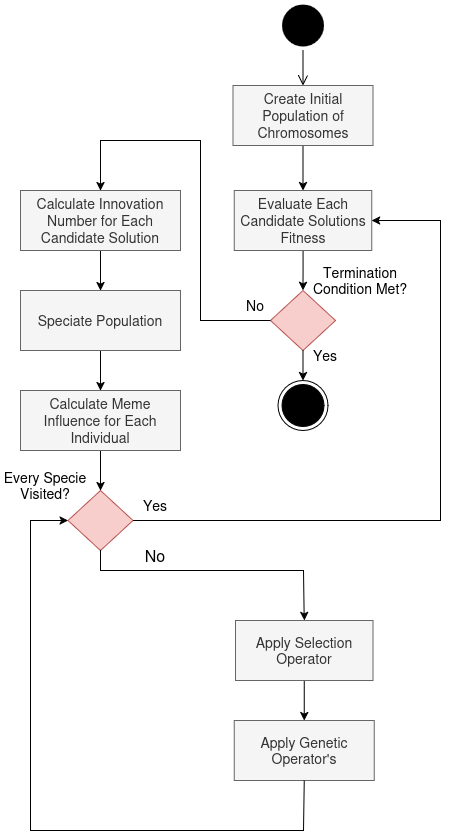
\includegraphics[width=0.65\textwidth]{Figures/chapter_gep_neat/gep_neat_framework.png} % Include the figure image
	\caption{Evolutionary Lifecycle of GEP-NEAT}
	\label{fig:gep_neat_framework} % Unique label used for referencing the figure in-text
\end{figure}

\parbreak\noindent At a high level, both NEAT and GEP follow a similar evolutionary cycle, that is, intialising a population, representing chromosomes, evaluating fitness, applying genetic operators, and iterating until a termination condition is met. The two approaches however diverge significantly in their internal mechanisms and innovations. NEAT introduces a sophisticated speciation mechanism, where historical gene information is tracked using innovation numbers. These are stored in a lookup table and used to calculate compatibility distance between individuals, allowing the population to be divided into species that evolve in parallel within their own niches (\cite{stanley2002evolving}).

\parbreak\noindent In contrast, GEP adheres more closely to the traditional genetic algorithm framework but distinguishes itself through a rich set of genetic operators that promote diversity and facilitate the emergence of reusable substructures, or building blocks, within chromosomes (\cite{ferreira2006gene}). Its use of Karva notation ensures syntactically valid expressions, making it particularly well-suited for evolving complex, non-linear representations.

\parbreak\noindent GEP-NEAT draws inspiration from both of these methodologies to form a unified framework, as illustrated in Figure \ref{fig:gep_neat_framework}. It leverages NEAT's innovation tracking and speciation to maintain diversity and protect novel structures, while adopting GEP's flexible chromosome representation to enable the evolution of expressive and structurally diverse neural networks.

\subsection{Representation}\label{sec:gep_neat_representation}
NEAT-GEP draws inspiration from the genotype-to-phenotype mapping introduced in Gene Expression Programming (GEP), particularly through the use of Karva notation, however, several modifications have been made to enhance the representation, starting with the adoption of prefix tree-style encoding. In traditional GEP, k-expressions are converted into expression trees by reading the linear string from left to right and top to bottom. While this method ensures syntactic correctness, it can become computationally expensive, especially when evaluating large populations or complex expressions since the expression tree must first be constructed from the expression string during each fitness evaluation. 

\parbreak\noindent As discussed in Chapter \ref{chapter:gep}, alternative encoding schemes such as prefix and postfix notation have been explored to address this limitation. On such approach, P-GEP, encodes linear chromosomes in prefix form. This representation improves the preservation of meaningful substructures during operations like crossover and mutation, which in turn supports more efficient and targeted exploration of the search space.

\parbreak\noindent Figure \ref{fig:gep_neat_p_gep} illustrates the differences between standard Karva notation and prefix notation, highlighting how subtrees - shown in purple, blue, and green - are affected by genetic operations. In standard Karva notation, these substructures are often disrupted during crossover, whereas prefix notation allows them to be preserved. For example, when a single-point crossover is applied between gene 3 and 4, the prefix-encoded chromosome maintains the integrity of its subtrees, whereas the same operation on a Karva-encoded chromosome may fragment them.

\parbreak
\begin{figure}[H] % Use [H] to suppress floating and place the figure/table exactly where it is specified in the text
	\centering % Horizontally center the figure on the page
	\includesvg[width=0.80\textwidth]{Figures/chapter_gep_neat/gep_neat_p_gep.svg} % Include the figure image
	\caption{GEP Encoding Scheme versus P-GEP Encoding Scheme}
	\label{fig:gep_neat_p_gep} % Unique label used for referencing the figure in-text
\end{figure}

\parbreak\noindent To illustrate how a GEP-NEAT chromosome is structured and functions, this chapter introduces a Simplified example. Consider a linear chromosome with a head size of $h = 3$ and a maximum function arity of $3$. Let the function set be ${D, T}$, where function $D$ takes two inputs and $T$ takes three, and the terminal set be ${a, b, c}$. According to GEP's formulation, the tail size is calculated using the formula:
\begin{ceqn}
	\begin{equation}
		t = h \times (n_{max} - 1) + 1 = 3 \times (3 - 1) + 1 = 7
	\end{equation}
\end{ceqn}

\noindent This results in a genome length of $h + t = 3 + 7 = 10$. In the original GEP formulation, both weight and threshold domains were encoded within the linear string. While threshold domains are useful in networks with binary or step activation functions, they can be restrictive in more expressive architectures. Therefore, in GEP-NEAT, only a weight domain is encoded, allowing for greater flexibility in network behaviour. The weight domain length is defined as:
\begin{ceqn}
	\begin{equation}
		D_w = h \times n_{max} = 3 \times 3 = 9
	\end{equation}
\end{ceqn}

\noindent A lookup weight array is used, where each gene in the weight domain serves as an index into this array. For example, a weight array of size $5$ might be defined as:
\begin{ceqn}
	\begin{equation}
		[-1.2, 2.3, 3.2, 4.4, -0.5, 6.0]
	\end{equation}
\end{ceqn}

\noindent A sample chromosome constructed using this configuration looks as follows:

\begin{ceqn}
	\begin{equation}\label{example:representation}
		\begin{array}{cccccccccccccccccc}
			0 & 1 & 2 & 3 & 4 & 5 & 6 & 7 & 8 & 9 & 0 & 1 & 2 & 3 & 4 & 5 & 6 & 7 \\
			D & a & T & a & b & c & a & b & a & 5 & 2 & 4 & 1 & 2 & 3 & 3 & 2 & 6
		\end{array}
	\end{equation}
\end{ceqn}

\noindent Based on the logic of GEP, to reiterate, genes 0 to 5 represent the actual expression tree, while genes 6 to 8 serve as buffer symbols that ensure syntactic correctness but do no contribute to the functional output. One notable limitation of the original GEP-NN implementation is the absence of bias nodes. While this omission had minimal impact in the original research likely due to the relatively constrained problems it had been applied to, its effect becomes more pronounced in larger and more complex solution spaces. In such cases, the lack of biasing can hinder the network's ability to shift activation thresholds, potentially leading to suboptimal performance. 

\parbreak\noindent To address this shortcoming, the first proposed novelty in GEP-NEAT is the explicit incorporation of bias into the chromosome structure. This is achieved by modifying the expression tree representation such that each function symbol encapsulates two components:
\begin{itemize}
    \item \textbf{bias enabled}: This stores a boolean value to determine whether a bias is enabled on the function symbol.
    \item \textbf{bias weight}: This stores the bias weight.
\end{itemize}

\parbreak\noindent Continuing with the illustrative example, let us now consider the bias values associated with the functional symbols in the expression string presented in Equation \ref{example:representation}:
\begin{itemize}
    \item Function Symbol \textbf{$D$}
    \begin{itemize}
        \item \textbf{bias enabled}: true
        \item \textbf{bias weight}: $0.4$
    \end{itemize}

    \item Function Symbol \textbf{$T$}
    \begin{itemize}
        \item \textbf{bias enabled}: false
        \item \textbf{bias weight}: $2.3$
    \end{itemize}
\end{itemize}

\parbreak\noindent This candidate solution corresponds to the expression tree, and by extension, the neural network depicted in Figure \ref{fig:gep_neat_representation_example_tree}. Similar to the forward propagation process in conventional neural networks, input values are assigned to the terminal $a$, $b$, and $c$, after which the expression tree is evaluated to compute the final network output.

\parbreak
\begin{figure}[H] % Use [H] to suppress floating and place the figure/table exactly where it is specified in the text
	\centering % Horizontally center the figure on the page
	\includesvg[width=0.8\textwidth]{Figures/chapter_gep_neat/gep_neat_representation_example_tree.svg} % Include the figure image
	\caption{Example GEP-NEAT Candidate Solution Expression Tree of Linear String in Equation \ref{example:representation}}
	\label{fig:gep_neat_representation_example_tree} % Unique label used for referencing the figure in-text
\end{figure}

\parbreak\noindent As illustrated in Figure \ref{fig:gep_neat_representation_example_tree}, the expression tree is decoded from the linear chromosome using prefix notation. Although a more detailed explanation is provided later in the chapter, it is import to note that weight values from the weight domain are assigned in a depth-first manner, progressing from leaves of the tree upward, similar to the evaluation strategy used in symbolic regression. Each weight value corresponds to an index in the predefined weight lookup array. Additionally, as previously mentioned, each function symbol in the tree is associated with a bias node. In this example the function symbol $D$ has its bias enabled, while $T$ does not, demonstrating how bias can be selectively applied within the network structure.

\parbreak\noindent Another limitation of the original GEP-NN algorithm lies in its restricted use of activation functions. As previously mentioned, the original implementation employed a threshold domain for each function symbol, where a neuron would output $0$ if its weighted sum of its inputs was below the associated threshold, and $1$ otherwise, effectively implementing a binary step function. Additionally, the only weighted sum operations used were linear in nature, represented by symbols such as $D$, $T$, and $Q$, with arities, $2$, $3$, and $4$ respectively.

\parbreak\noindent While this approach was sufficient for the original problem domains, it proved inadequate for more complex tasks such as symbolic regression and classification. Subsequent research demonstrated that by modifying these function symbols to represent arithmetic operations like subtraction, multiplication, and division, the algorithm's expressiveness could be significantly improved (\cite{improvedGepnn}). This however still did not address the broader limitation of lacking non-linear activation functions, which are a fundamental component of modern neural networks.

\parbreak\noindent To overcome this, the next proposed novelty in GEP-NEAT framework is the introduction of configurable activation functions. At each function node, the weighted sum - computed as the sum of all inputs plus the bias - is passed through an activation function specific to that symbol. This allows each function symbol to encode not only its arity and operation but also its own activation behaviour. The function set is fully configurable, enabling the inclusion of a diverse range of activation functions (e.g., sigmoid, tanh, ReLU), each associated with different arities. This design mirrors the flexibility of traditional neural networks, allowing GEP-NEAT to learn which activation functions are most effective for a given problem domain.

\subsection{Initial Population}
\noindent In the original GEP algorithm, Ferreira proposed a start-up protocol designed to accelerate the evolutionary search process by ensuring that the initial population includes at least one viable candidate solution, that is, one with a fitness value above a minimum threshold (\cite{ferreira2006gene}). The rationale behind this approach is to establish a lineage from a single, functional founder, thereby promoting faster convergence through a more directed exploration-exploitation balance. This strategy however introduces a potential drawback, that is, it increases the risk of premature convergence, where the population may stagnate around local optima due to limited initial diversity.

\parbreak\noindent In contrast, the NEAT algorithm adopts a different philosophy known as starting out minimally mentioned in Chapter \ref{sec:ne_neat}. During intialisation, NEAT generates networks with no hidden nodes, resulting in the simplest possible structures. This minimalist design encourages the discovery of compact and efficient solutions in low-dimensional spaces, which can lead to performance gains (\cite{stanley2002evolving}). A common concern with this approach is that structural innovations such as the addition of new nodes or connections may be lost early in evolution. NEAT addresses this by introducing innovation numbers, which track historical gene changes and enable the algorithm to protect and preserve novel topological features through speciation.

\parbreak\noindent The proposed GEP-NEAT framework does not adopt GEP's start-up control mechanism. Instead, it incorporates NEAT's minimalist intialisation strategy to mitigate the risk of premature convergence. During the intialisation phase, individuals are generated with only a single function symbol positioned at the root of the linear chromosome. This ensures that the initial population consists of structurally simple candidates, allowing complexity to emerge gradually through evolutionary processes. An example of such an initial chromosome is shown in Equation \ref{example:gep_neat_initial}, with its corresponding phenotype representation illustrated in Figure \ref{fig:gep_neat_initial_example}.
\begin{ceqn}
	\begin{equation}\label{example:gep_neat_initial}
		\begin{array}{cccccccccccccccccc}
			0 & 1 & 2 & 3 & 4 & 5 & 6 & 7 & 8 & 9 & 0 & 1 & 2 & 3 & 4 & 5 & 6 & 7 \\
			D & a & b & a & b & c & a & b & a & 5 & 2 & 4 & 1 & 2 & 3 & 3 & 2 & 6
		\end{array}
	\end{equation}
\end{ceqn}

\parbreak
\begin{figure}[H] % Use [H] to suppress floating and place the figure/table exactly where it is specified in the text
	\centering % Horizontally center the figure on the page
	\includesvg[width=0.6\textwidth]{Figures/chapter_gep_neat/gep_neat_initial_example.svg} % Include the figure image
	\caption{Example GEP-NEAT Candidate Solution Expression Tree of Linear String in Equation \ref{example:representation} Generated Through Initialisation Phase}
	\label{fig:gep_neat_initial_example} % Unique label used for referencing the figure in-text
\end{figure}

\parbreak\noindent As a result, the initial population consists of genotypes that encode networks with only an input and output layer, excluding any hidden layers. This design choice is consistent with NEAT's underlying philosophy, which advocates for beginning the evolutionary process in the simplest possible solution space. By doing so, structural innovations are allowed to emerge gradually, enabling the algorithm to discover increasingly complex and effective architectures over time.

\subsection{Evaluating Candidate Solutions}
As outlined in Section \ref{sec:gep_neat_representation}, candidate solutions in GEP-NEAT are represented as linear string in their genotype form and are translated into corresponding expression trees (i.e., neural networks) using prefix notation. While this genotype-to-phenotype mapping is essential for evaluating network behaviour, it can become computationally expensive, particularly when dealing with complex linear strings and large populations across many generations.

\parbreak\noindent To address this challenge, the S\_GEP algorithm, an extension of P-GEP, offers a significant advantage by enabling the evaluation of expression strings without converting them into expression trees. Although S\_GEP has not yet been applied in the context of GEP-NN, its integration into GEP-NEAT is motivated by the need to reduce the computational overhead associated with repeated forward evaluations during fitness calculation. As discussed in Chapter \ref{sec:gep_current_research}, S\_GEP's approach is particularly beneficial when combined with enhancements such as activation functions and bias nodes, which slightly modify the original evaluation process.

\parbreak\noindent In this modified framework, evaluation begins by substituting terminal symbols with actual input values. For instance, when evolving a network to solve the XOR problem, the four input combinations, $00$, $01$, $10$, and $11$, are sequentially fed into the network. Each input replaces the corresponding terminal symbol (e.g., \textit{a} and \textit{b}) in the expression string. To ensure that only the coding region of the chromosome is evaluated, the effective gene length must first be determined. This is computed using the procedure outlined in Algorithm \ref{alg:gep_neat_el}, which identifies the portion of the linear string that contributes to the final output.

\parbreak
\begin{algorithm}
	\caption{Effective gene length (adapted from \cite{peng2014improved})}\label{alg:gep_neat_el}
	\begin{algorithmic}[1]
	% \Ensure $y = x^n$
	\item \textbf{Input}: String of gene symbols
	\item \textbf{Output}: eL
	\item Initialize variables $Len=1$ and $count=0$
	\item \textbf{while} scanning gene symbols starting from left to right:
	\item \quad $Len = Len + 1$;
	\item \quad \textbf{if} current gene symbol is function:
	\item \quad \quad $count = count - 1$
	\item \quad \textbf{else}:
	\item \quad \quad $count = count - 1$
	\item \quad \textbf{if} $count < 0$:
	\item \quad \quad return $eL=Len$ as output
\end{algorithmic}
\end{algorithm}

\parbreak\noindent Once the effective gene length has been determined, the linear chromosome can be evaluated directly using Polish notation, as the encoding follows a prefix format. This allows for a systematic traversal of the expression string without the need to construct an intermediate expression tree. The evaluation process is carried out using the procedure outlined in Algorithm \ref{alg:gep_neat_evaluate}, which processes the linear string to compute the final output of the candidate solution.

\parbreak
\begin{algorithm}
	\caption{GEP-NEAT Evaluation Algorithm (inspired from \cite{peng2014improved})}\label{alg:gep_neat_evaluate}
	\begin{algorithmic}[1]
	\item Calculate eL using Algorithm \ref{alg:gep_neat_el}
	\item set \textit{stack} array variable to an empty list
	\item set \textit{weight\_index} variable to 0
	\item \textbf{while} reading effective gene from right to left using eL:
	\item \quad \textbf{if} current gene is a terminal symbol:
	\item \quad \quad push terminal symbol on stack
	\item \quad \textbf{else if} current gene is function symbol:
	\item \quad \quad set \textit{weighted\_sum} variable to 0
	\item \quad \quad \textbf{for} number of function symbol inputs:
	\item \quad \quad \quad pop value from stack and multiply with weight from weight lookup array at index \textit{weight\_index}
	\item \quad \quad \quad add result value to \textit{weighted\_sum}
	\item \quad \quad \quad increment \textit{weight\_index} by 1
	\item \quad \quad \textbf{if} bias is enabled for current function symbol:
	\item \quad \quad \quad add function symbol's bias value to \textit{weighted\_sum}
	\item \quad \quad apply function symbol's activation function to \textit{weighted\_sum}
	\item \quad \quad push result value onto stack
	\item pull value from stack and return
\end{algorithmic}
\end{algorithm}

\parbreak\noindent Once the linear string has been evaluated, the resulting output is passed into a fitness function to compute a corresponding fitness value. Fitness functions are inherently problem-specific, designed to quantify how well a candidate solution performs in relation to the task at hand. For example, in both NEAT and GEP implementations of the XOR problem, a commonly used fitness function is defined as shown in Equation \ref{alg:absolute_error}.
\begin{ceqn}
	\begin{equation}\label{alg:absolute_error}
		f_{i} = \sum_{j=1}^{C_t}(M-|C_{(i,j)}-T_{(j)}|
	\end{equation}
\end{ceqn}

\noindent where:
\begin{itemize}
    \item $f_i$ is fitness for candidate solution $i$
    \item $C_t$ is the number of test cases
    \item $M$ is the maximum value for a fitness case
    \item $C_{(i,j)}$ is the value returned by individual $i$ for case $j$
    \item $T_{(j)}$ is the target value for case $j$
\end{itemize}

\parbreak\noindent In other problem domain, such as the CartPole balancing task, fitness functions are typically based on a reward-based scheme. In this setup, the agent receives a predefined reward for each time step that the pole remains balanced during an episode. If the pole falls or the episode terminates prematurely, the reward drops to zero. This incentivises the agent to maintain balance for as long as possible, guiding the evolutionary process toward more stable and effective control strategies.

\subsection{Speciation}
The next phase of the algorithm involves two key operations namely, calculating innovation numbers and performing speciation. In the NEAT algorithm, innovation numbers serves as a mechanism to track the historical origin of genes. This tracking is crucial for preserving novel structures during evolution. NEAT maintains a global innovation number table. Whenever a new, previously unseen connection between two nodes is introduces, the global innovation number is incremented and assigned to that connection. This system allows for meaningful comparisons between genomes by identifying matching and non-matching genes based on their innovation numbers. As discussed in Chapter \ref{sec:ne_neat}, this comparison is essential for determining genetic similarity and enabling speciation, grouping similar genomes into species to protect innovation.

\parbreak\noindent GEP-NEAT extends this concept by redefining what innovation numbers represent. Instead of tracking individual connections, GEP-NEAT assigns innovation numbers to entire subtrees within an expression tree. Each unique subtree is treated as a distinct innovation, and thus receives its own innovation number. 

\parbreak\noindent During evaluation, the expression tree is traversed in the same order as it would be during execution. As values are pushed onto the stack, each subtree is examined. The algorithm checks whether the subtree already exists in a global innovation number lookup table. If it does not, the corresponding innovation number is reused. If not, the subtree is added to the table and assigned a new, incremented innovation number. This process is visually illustrated in Figure \ref{fig:gep_neat_innovation_number}, and the detailed mechanism is outlined in Algorithm \ref{alg:gep_neat_innovation_number}.

\parbreak
\begin{figure}[H] % Use [H] to suppress floating and place the figure/table exactly where it is specified in the text
	\centering % Horizontally center the figure on the page
	\includesvg[width=\textwidth]{Figures/chapter_gep_neat/gep_neat_innovation_number.svg} % Include the figure image
	\caption{Innovation Number Assignment on GEP-NEAT Expression Tree}
	\label{fig:gep_neat_innovation_number} % Unique label used for referencing the figure in-text
\end{figure}

\parbreak
\begin{algorithm}
	\caption{GEP-NEAT Innovation Number Algorithm}\label{alg:gep_neat_innovation_number}
	\begin{algorithmic}[1]
	\item Calculate eL using Algorithm \ref{alg:gep_neat_el}
	\item set \textit{stack} array variable to an empty list
	\item \textbf{while} reading effective gene from right to left using eL:
	\item \quad \textbf{if} current gene is a terminal symbol:
	\item \quad \quad push terminal symbol on stack
	\item \quad \textbf{else if} current gene is function symbol:
	\item \quad \quad push current function symbol to stack
	\item \quad \quad access index [function symbol's arity plus 1] from stack to get subtree
	\item \quad \quad set \textit{innovation\_number} variable to 0
	\item \quad \quad \textbf{if} innovation number does not exist in lookup table:
	\item \quad \quad \quad set \textit{innovation\_number}  to length of lookup table minus 1
	\item \quad \quad \textbf{else}:
	\item \quad \quad \quad set \textit{innovation\_number} variable to found value in lookup table
	\item \quad \quad push \textit{innovation\_number} to stack
\end{algorithmic}
\end{algorithm}

\parbreak\noindent Innovation numbers in GEP-NEAT serve as a system for encoding subtree configurations, which can collectively represent entire expression trees. Each expression tree can be described by its innovation number composition, a list of innovation numbers corresponding to the subtrees to the subtrees that make up the tree.

\parbreak\noindent Each innovation number in this composition list is associated with a specific subtree and its corresponding weights. Conceptually, this composition list functions as a mapping - the key is the innovation number, and the value is a tuple containing the subtree structure and its associated weights. This structure representation enables sufficient comparison, storage, and manipulation of expression trees. The process of generating the innovation number is detailed in Algorithm \ref{alg:gep_neat_innovation_number_composition}. For instance, the expression tree illustrated in Figure \ref{fig:gep_neat_innovation_number} has its corresponding number composition shown in Figure \ref{fig:gep_neat_innovation_number_composition}.

\parbreak
\begin{algorithm}
	\caption{GEP-NEAT Innovation Number Composition Algorithm}\label{alg:gep_neat_innovation_number_composition}
	\begin{algorithmic}[1]
	\item Calculate eL using Algorithm \ref{alg:gep_neat_el}
	\item set \textit{weight\_index} variable to 0
	\item set \textit{stack} array variable to an empty list
	\item \textbf{while} reading effective gene from right to left using eL:
	\item \quad \textbf{if} current gene is a terminal symbol:
	\item \quad \quad push terminal symbol on stack
	\item \quad \textbf{else if} current gene is function symbol:
	\item \quad \quad set \textit{weights} array variable to empty list
	\item \quad \quad \textbf{for} number of function symbol inputs:
	\item \quad \quad \quad retrieve value from weight lookup array indexed at current input and add to weight array
	\item \quad \quad \quad increment \textit{weight\_index} by 1
	\item \quad \quad append  current symbol to stack
	\item \quad \quad access index [function symbol's arity plus 1] from stack to get subtree
	\item \quad \quad get innovation number using subtree from lookup table
	\item \quad \quad append innovation number with its corresponding subtree and \textit{weights} to the \textit{innovation\_number\_composition}
	\item \quad \quad push result value onto stack
	\item return \textit{innovation\_number\_composition}
\end{algorithmic}
\end{algorithm}

\parbreak
\begin{figure}[H] % Use [H] to suppress floating and place the figure/table exactly where it is specified in the text
	\centering % Horizontally center the figure on the page
	\includesvg[width=\textwidth]{Figures/chapter_gep_neat/gep_neat_innovation_number_composition.svg} % Include the figure image
	\caption{Innovation Number Composition Expression Tree in Figure \ref{fig:gep_neat_innovation_number}}
	\label{fig:gep_neat_innovation_number_composition} % Unique label used for referencing the figure in-text
\end{figure}

\parbreak\noindent To group similar solutions and protect structural innovations during evolution. GEP-NEAT employs the same speciation mechanism used in NEAT, based on a compatibility distance function. This function measures the genetic similarity between individuals, allowing the algorithm to cluster them into species. Inspired by NEAT, GEP-NEAT introduces its own version of the compatibility distance function, tailored to its subtree-based innovation number system:
\begin{ceqn}
	\begin{equation}\label{alg:speciation}
		\delta = \frac{c_1NM}{N} + c_2\cdot{\overline{W}}
	\end{equation}
\end{ceqn}

\noindent where:
\begin{itemize}
    \item $\delta$ is the compatibility distance between a pair of genomes
    \item $NM$ is the number of non-matching genes
    \item $\overline{W}$ is the average weight difference of matching gene arrays
    \item $N$ is the number of genes in the larger genome (serving as a normalization)
    \item $c_1$ and $c_2$ serve as adjustments in the importance of the two factors
\end{itemize}

\parbreak\noindent In the original NEAT paper, disjoin and excess genes were defines as separate categories of non-matching genes, however, these distinctions did not carry unique implications in terms of how they influenced the algorithm's behaviour. Recognising this, GEP-NEAT simplifies the classification by focusing on two categories, matching and non-matching genes.

\parbreak\noindent A key difference in GEP-NEAT lies in how it handles weight difference between genes. Even when two genes represent the same subtree configuration, they may have different weights associated with the same connections. Therefore, when calculating the average weight difference, GEP-NEAT compares only the weights of matching genes, those that share the same subtree structure. The method for computing this average weight difference is outlines as follows:
\begin{ceqn}
	\begin{equation}\label{alg:weight_difference}
		\overline{W} = \frac{\sum_{j=0}^{N}|W_{aj} - W_{bj}|}{N}
	\end{equation}
\end{ceqn}

\noindent where:
\begin{itemize}
	\item $\overline{W}$ is the average weight difference of the subtree
	\item $N$ is the number of child nodes in the subtree
	\item $W_{aj}$ is the weight of subtree '$a$' of child node $j$
	\item $W_{bj}$ is the weight of subtree '$b$' of child node $j$
\end{itemize} 

\parbreak
\begin{figure}[H] % Use [H] to suppress floating and place the figure/table exactly where it is specified in the text
	\centering % Horizontally center the figure on the page
	\includesvg[width=\textwidth]{Figures/chapter_gep_neat/gep_neat_innovation_number_compare.svg} % Include the figure image
	\caption{Comparing Expression Trees Using Innovation Number Compositions}
	\label{fig:gep_neat_innovation_number_compare} % Unique label used for referencing the figure in-text
\end{figure}

\parbreak\noindent The number of matching and non-matching genes between two expression trees can be determined by first converting each tree into its corresponding innovation number composition. Once in this form, it becomes straightforward to compare the sets of innovation numbers and identify which genes are shared and which are unique to each tree. As illustrated in Figure \ref{fig:gep_neat_innovation_number_compare}, the matching genes between expression tree 1 and expression tree 2 are $\{2\}$, while the non-matching genes are $\{1, 3, 4, 5\}$.

\parbreak\noindent Speciation in GEP-NEAT occurs during every evolutionary generation and follows the procedure outlined in Algorithm \ref{alg:speciation_2}. At the start of each generation, the population is randomly shuffled to ensure that every individual has a fair chance of becoming a species representative. This shuffling helps improve the grouping of individuals into species by avoiding bias from fixed representatives.

\parbreak
\begin{algorithm}[H]
	\caption{GEP-NEAT Speciation Algorithm}\label{alg:speciation_2}
	\begin{algorithmic}[1]
	\item Initialise empty list of \textit{species}
	\item Shuffle the population
	\item \textbf{for} every individual in population:
	\item \quad \textbf{if} species is empty:
	\item \quad \quad add individual as first specie group
	\item \quad \textbf{else}:
	\item \quad \quad \textbf{for} every specie in the \textit{species} list:
	\item \quad \quad \quad calculate compatibility distance between representative individual in current specie and current individual
	\item \quad \quad \quad \textbf{if} compatibility distance is less than compatibility threshold $\delta_{ct}$:
	\item \quad \quad \quad \quad add individual to current specie
	\item \quad \quad \quad \quad \textbf{break} to next individual
\end{algorithmic}
\end{algorithm}

\parbreak\noindent Each individual in the population is then compared against the representative of every existing species. If the compatibility distance between the individual and a species representative is less than a compatibility threshold $\delta_{ct}$, the individual is assigned to that species. This comparison continues until all individuals have been assigned to a species group. This dynamic grouping mechanism helps maintain diversity and protects innovative structures by allowing similar individuals to evolve together within their respective species.

\subsection{Meme Influence}
Richard Dawkins, a British evolutionary biologist, is widely known for his gene-centered view of evolution, most notably presented in his 1976 book \textit{The Selfish Gene} (\cite{dawkins1981selfish}). In this work, Dawkins argues that genes are the fundamental units of natural selection, driving evolutionary change through processes of replication and competition. He also introduces the concept of the "meme", a cultural counterpart to biological genes. A meme represents a unit of culture transmission, such as an idea, behaviour, or trend, which spreads through imitation. Like genes, memes undergo variation, competition, and selection, making them subject to evolutionary dynamics.

\parbreak\noindent Building on this idea, GEP-NEAT levarages its innovation tracking system to introduce a novel concept called meme influence. Since subtree configurations are recorded in a global innovation lookup table throughout the evolutionary process, GEP-NEAT uses this structure to monitor and rank the impact of different subtrees. Two additional attributes are tracked for each innovation number, namely, the innovation number composition, and the meme influence.

\parbreak\noindent These attributes help evaluate the significance of each subtree configuration in contributing to the overall fitness of individuals. The process begins by calculating the innovation contribution of each innovation number based on the adjusted fitness of the individual within its species, as described in Equation \ref{equation:innovation_contribution}.

\parbreak\noindent Each innovation number that appears in an individual's composition receives an increment to its contribution score, reflecting its role in producing high-fitness individuals. Although Equation \ref{equation:innovation_contribution} assumes equal contribution from all innovation numbers, aggregating these values across the population allows frequently successful subtrees to accumulate higher scores.

\parbreak
\begin{algorithm}[H]
	\caption{GEP-NEAT Meme Influence Algorithm}\label{alg:meme_influence}
	\begin{algorithmic}[1]
	\item \textbf{for} specie in species:
	\item \quad \textbf{for} individual in specie:
	\item \quad \quad calculate \textit{innovation contribution} using Equation \ref{equation:innovation_contribution}
	\item \quad \quad \textbf{for} each innovation number in the current individual's innovation number composition:
	\item \quad \quad \quad innovation\_lookup\_table[innovation number][innovation contribution attribute] += \textit{innovation contribution}
	
	\item 

	\item \textbf{for} each innovation number in innovation\_lookup\_table:
	\item \quad calculate the normalised value for the current innovation number using Equation \ref{equation:normalise}
	\item \quad calculate innovation number contribution using Equation \ref{equation:innovation_contribution}
	\item \quad calculate the \textit{meme influence} for the current individual using Equation \ref{equation:meme_influence}
	\item \quad append the \textit{meme influence} value as attribute to the current innovation number
\end{algorithmic}
\end{algorithm}

\parbreak\noindent Once all innovation contributions have been updates, they are normalised using Equation \ref{equation:normalise}, enabling consistent ranking across generations. The meme influence for an individual \textit{i} is then calculated using Equation \ref{equation:meme_influence}, which incorporates a decay rate parameter $\alpha$. This calculation uses shifting average moving function, inspired by the work of Haynes (\cite{haynes2012exponential}), to emphasise current trends while allowing outdated patterns to gradually fade. The result is a dynamic ranking system that identifies which innovation numbers (i.e., subtree configurations) are most influential in driving evolutionary success within each generation.

\parbreak
\begin{ceqn}
\begin{equation}\label{equation:innovation_contribution}
    innovation\:contribution = \frac{individual\:adjusted\:fitness}{length(individual\:innovation\:number\:composition)}
\end{equation}
\end{ceqn}

\parbreak
\begin{ceqn}
	\begin{equation}\label{equation:normalise}
		normalised\:value_i = \frac{innovation\:contribution_i - min\:innovation\:contribution}{max\:innovation\:contribution - min\:innovation\:contribution}
	\end{equation}
\end{ceqn}

\parbreak
\begin{ceqn}
	\begin{equation}\label{equation:meme_influence}
		meme\:influence_i = (\alpha \times normalised\:value) + ((1 - \alpha) \times meme\:influence_i)
	\end{equation}
\end{ceqn}

\subsection{Selection}
Both GEP and NEAT utilise well-established selection mechansims in evolutionary computation. NEAT typically employs tournament selection, while GEP uses roulette wheel selection. A limitation of these traditional methods however rely solely on fitness score to guide selection, without considering the structural innovations that contribute to an individual's success.

\parbreak\noindent To address this, GEP-NEAT introduces a more nuanced approach by incorporating the meme influence metric, an attribute tracked for each innovation number that reflects its historical contribution to high-performing individuals. This enables the algorithm to rank innovation numbers based on their evolutionary impact. Building on this idea, GEP-NEAT proposes a novel selection operator called Meme Influence Roulette Wheel Selection (MIRWS). While it is inspired by standard roulette wheel selection, the key diffence is that meme influence values are used in place of raw fitness scores. This allows the selection process to favour individuals composed of highly influential subtrees, rather than just those with high fitness in the current generation.

\parbreak\noindent The adjusted fitness scores based on meme influence are computed using Algorithm \ref{alg:mirws} after which the standard roulette wheel selection procedure is applied using these adjusted values.

\parbreak
\begin{algorithm}[H]
	\caption{GEP-NEAT Meme Influence Roulette Wheel Selection Algorithm}\label{alg:mirws}
	\begin{algorithmic}[1]
	\item \textbf{for} each individual in the population:
	\item \quad initialise \textit{total\_individual\_fitness} variable to 0
	\item \quad \textbf{for} each innovation number in the current individual's innovation number composition:
	\item \quad \quad \textit{total\_individual\_fitness} += current innovation numbers meme influence value
	\item \quad set the current individuals adjusted fitness to the \textit{total\_individual\_fitness}
	\item
	\item intialise \textit{selected\_individual} array to empty list
	\item \textbf{for} number of individuals required:
	\item \quad choose a random number between 0 and the total adjusted fitness based on the meme influence value
	\item \quad set \textit{current} variable to 0
	\item \quad \textbf{for} every individual in the population:
	\item \quad \quad \textit{current} += current individuals adjusted fitness
	\item \quad \quad \textbf{if} \textit{current} >= random number chosen:
	\item \quad \quad \quad append current individual to \textit{selected\_individual} list
	\item \textbf{return} \textit{selected\_individual}
\end{algorithmic}
\end{algorithm}

\subsection{Genetic Operators}
Once individuals are selected from each species during every generation of the evolutionary process, they are given the opportunity to undergo genetic variation through mutation and crossover to produce offspring. GEP-NEAT supports a variety of genetic operators each associated with its own probability.

\parbreak\noindent Among these, mutation is the most critical operator and is implemented across multiple domains that make up the chromosome. Since the genotype in GEP-NEAT is primarily structured using Karva notation, a linear representation of expression trees, many of the mutation operators are adapted from traditional GEP techniques. In addition, GEP-NEAT introduces new mutation strategies that are influenced by the concept of meme influence, allowing the algorithm to bias variance toward subtrees that have historically contributed to higher fitness.

\parbreak\noindent These diverse mutation and crossover mechanisms enable GEP-NEAT to explore the search space effectively while preserving and promoting structure innovations.

\subsubsection{Neuron Mutation}
This mutation mechanisms, governed by a mutation rate denoted as $\rho_{neuron}$, targets the neuron portion of the expression string using an n-point mutation strategy. In this approach, $n$ random genes are selected within the expression string for mutation.

\parbreak\noindent The behaviour of the mutation depends on the position of the gene within the expression string, which follows the structure of Karva notation:
\begin{itemize}
	\item If the mutation point is located at the root (i.e, the first symbol which is a function symbol), the mutated gene must also be a function symbol to preserve syntactic validity.
	\item If the mutation occurs within the head of the expression string (excluding the root), the gene can be mutated into either a function or a terminal symbol, maintaining flexibility while ensuring structural correctness.
	\item If the mutation point lies within the tail of the expression string, only terminal symbols are allowed, as this region acts as a buffer.
\end{itemize}

\parbreak\noindent This structured mutation approach ensures that resulting expression trees remain syntactically valid while introducing meaningful variation into the population.

\subsubsection{Weight Mutation}
This mutation mechanism, controlled by the mutation rate $\rho_{weight}$, targets the weight portion of the expression string using an n-point mutation strategy. In this process, $n$ random weight genes are selected for mutation.

\parbreak\noindent Each selected weight gene is then reassigned a new value, which is randomly and uniformly drawn from the range defined by the index size of the weight lookup array. This ensures that the mutation weights remain valid and introduces a mechanism in which the resulting neural network can test out different weights between neurons.

\subsubsection{Weight Lookup Mutation}
This mutation mechanism, governed by the mutation rate $\rho_{weight\_lookup}$, targets the weight lookup array using an n-point mutation strategy. In this process, $n$ random entries within the weight lookup array are selected for mutation.

\parbreak\noindent Each selected weight value is then replaced with a new value, drawn from a uniform distribution, ensuring that the updated weights remain within a valid and diverse range. This mutation allows the algorithm to explore alternative weight configurations, influencing how subtrees are evaluated across individuals.

\subsubsection{Bias Mutation}
As previously discussed, the introduction of bias in GEP-NEAT involves two key attributes:
\begin{itemize}
	\item A bias toggle, which determines whether bias is enabled for a given function symbol.
	\item A bias value, which specifies the magnitude or direction of the bias.
\end{itemize}

\parbreak\noindent Each of these attributes has its own dedicated mutation mechanism:
\begin{itemize}
	\item \textbf{Bias Toggle Mutation}: Controlled by the mutation rate $\rho_{bias\_toggle}$, this mutation randomly selected a function symbol within a chromosome and flips the state of its bias toggle. This is effectively a bit-flip operation, switching the toggle between true and false, thereby enabling or disabling the bias for that function.
	\item \textbf{Bias Value Mutation}: Governed by the mutation rate $\rho_{bias}$, this mutation targets the bias value of a randomly chosen function symbol. The value is then mutated using a uniform distribution. This allows for controlled variability in the strength or direction of the bias applied.
\end{itemize}

\subsubsection{Inversion}
Inversion is a genetic operator designed to introduce structural diversity by selecting two points within a chromosome and reversing the sequence of genes between them. This operation aims to explore new regions of the search space that may not be reachable through standard mutation or crossover alone.

\parbreak\noindent GEP-NEAT implements two types of inversion operators, each applied to a different domain of the chromosome:
\begin{itemize}
	\item \textbf{Neuron inversion}, with a mutation probability of $\rho_{inversion\_neuron}$, targets the neuron portion of the chromosome.
	\item \textbf{Weight inversion}, with a mutation probability of $\rho_{inversion\_weight}$, operates on the weight portion.
\end{itemize}

\parbreak\noindent A critical constraint is enforced during neuron inversion to maintain syntactic correctness. If the first target site selected for inversion is the root of the expression tree, then the second target site must also contain a function symbol. This ensures that the resulting expression remains valid after inversion. If this condition is not met, new target sites are selected until the constraint is satisfied.

\subsubsection{Transposition}
Transposition is a genetic operator inspired by biological processes, where segments of genetic material known as insertion sequences (IS elements), are relocated to different positions within a chromosome. In GEP-NEAT, transposition is used not only to introduce structural diversity but also to encourage the emergence of repeatable and reusable structures within individuals. This can lead to the discovery of modular building blocks that contribute to evolutionary sucess.

\parbreak\noindent GEP-NEAT implements five types of transposition operators, adapted from traditional GEP:
\begin{itemize}
	\item \textbf{IS Transposition}: With a probability of $\rho_{is}$, this operator selects two random target sites within the neuron domain of the expression string. The segment between these sites forms the IS element, which may begin with either a function or terminal symbol. This IS element is then inserted into the head of the expression string (excluding the root), promoting structural variation while maintaining syntactic correctness.
	\item \textbf{RIS Transposition}: Governed by the probability $\rho_{ris}$, this operator selects a Root Insertion Sequence (RIS) by choosing two target sites such that the first site contains a function symbol. The resulting RIS element is then transposed to the root of the expression string, directly modifying the top-level structure of the expression tree.
	\item \textbf{Gene Transposition}: With a probability of $\rho_{gis}$, this operator transposes an entire gene from one location in the chromosome to another. This allows for large-scale rearrangements, potentially enabling the reuse of effective gene structures across different contexts.
	\item \textbf{Weight Transposition}: Controlled by the probability $\rho_{wis}$, this operator selects a Weight Insertion Sequence (WIS) by choosing two random target sites within the weight domain of the chromosome. The WIS segment is then transposed to a new location within the weight domain, allowing for flexible reconfiguration of weight patterns.
	\item \textbf{Meme Influence Sequence Transposition (MIIST)}: Introduced specifically in GEP-NEAT, this novel operator operates with a mutation rate of $\rho_{miis}$. MIIST is inspired by IS and RIS transposition but leverages the meme influence metric to guide the operation. It works by identifying the highest-performing subtree configuration (i.e., the innovation number with the greatest meme influence) and transposing it into a randomly selected function symbol location within another individual. This mechanism encourages the spread of emergent trends within the population, promoting convergence toward effective building blocks.
\end{itemize}

\parbreak\noindent By enabling the relocation and reuse of function components, transposition supports the formation of modular, repeatable structures, a key factor in building scalable and generalisable solutions in evolutionary computation.

\subsubsection{Recombination}
GEP-NEAT, like traditional GEP, is built upon Karva notation, which provides a structured and linear representation of expression trees. One of the key advantages of this representation is that it enables crossover operations to be performed naturally and efficiently. In GEP-NEAT, two primary crossover mechanisms are supported:
\begin{itemize}
	\item \textbf{One-Point Crossover}: A crossover mechanism with probability $\rho_{one\_point}$, where a single crossover point is randomly chosen between two parent chromosomes. The genetic material beyond this point is then exchanged between the two individuals, producing two offspring. This process is illustrated in Figure \ref{fig:singlepoint}.
	\item \textbf{Two-Point Crossover}: A crossover mechanism with probability $\rho_{two\_point}$, where two crossover points are selected, and the segment between them is swapped between the two parents. This allows for more substantial recombination of genetic material. A visual example of this operation is shown in Figure \ref{fig:multipoint}.
\end{itemize}

\parbreak\noindent These crossover operations can be generalised into n-point crossover, where multiple segments are exchanged, though this is typically treated as a higher-level abstraction. Importantly, GEP-NEAT applies crossover across both domains of the chromosome, that is, the neuron domain and weight domain. To facilitate this, the expression string is organised such that the neuron genes are prefixed, followed by the weight genes as a suffix (forming the fully qualified expression string). This layout ensures that crossover can be performed seamlessly across both domains, preserving the integrity of the genotype while enabling rich genetic variation.

\subsection{Termination Conditions}
At some point, the evolutionary process must be terminated once a sufficiently refined solution has been found. In evolutionary algorithms, including GEP-NEAT, there are several strategies for determining when to stop the algorithm. In GEP-NEAT, two primary termination conditions are used:
\begin{itemize}
	\item \textbf{Maximum Generation Limit}: A predefined limit is set on the number of generations the algorithm is allowed to run. This ensures that the evolutionary process does not continue indefinitely and provides a safeguard against excessive computation.
	\item \textbf{Fitness-Based Termination}: The algorithm also monitors the best-performing individual in the population. If this individual's fitness meets or exceeds the maximum fitness threshold defined for the problem, the algorithm concludes that an optimal or sufficiently good solution has been found and terminates early.
\end{itemize}

\parbreak\noindent The evolutionary process halts as soon as either of these conditions is satisfied, ensuring a balance between computational efficiency and solution quality.

\section{Prototype Implementation}\label{sec:gep_neat_protoype_implementation}
Richard Dawkins, 


\section{Model Validation and Results}\label{sec:gep_neat_model_validation}
Hello